% Options for packages loaded elsewhere
\PassOptionsToPackage{unicode}{hyperref}
\PassOptionsToPackage{hyphens}{url}
%
\documentclass[
  ignorenonframetext,
]{beamer}
\usepackage{pgfpages}
\setbeamertemplate{caption}[numbered]
\setbeamertemplate{caption label separator}{: }
\setbeamercolor{caption name}{fg=normal text.fg}
\beamertemplatenavigationsymbolsempty
% Prevent slide breaks in the middle of a paragraph
\widowpenalties 1 10000
\raggedbottom
\setbeamertemplate{part page}{
  \centering
  \begin{beamercolorbox}[sep=16pt,center]{part title}
    \usebeamerfont{part title}\insertpart\par
  \end{beamercolorbox}
}
\setbeamertemplate{section page}{
  \centering
  \begin{beamercolorbox}[sep=12pt,center]{part title}
    \usebeamerfont{section title}\insertsection\par
  \end{beamercolorbox}
}
\setbeamertemplate{subsection page}{
  \centering
  \begin{beamercolorbox}[sep=8pt,center]{part title}
    \usebeamerfont{subsection title}\insertsubsection\par
  \end{beamercolorbox}
}
\AtBeginPart{
  \frame{\partpage}
}
\AtBeginSection{
  \ifbibliography
  \else
    \frame{\sectionpage}
  \fi
}
\AtBeginSubsection{
  \frame{\subsectionpage}
}
\usepackage{lmodern}
\usepackage{amssymb,amsmath}
\usepackage{ifxetex,ifluatex}
\ifnum 0\ifxetex 1\fi\ifluatex 1\fi=0 % if pdftex
  \usepackage[T1]{fontenc}
  \usepackage[utf8]{inputenc}
  \usepackage{textcomp} % provide euro and other symbols
\else % if luatex or xetex
  \usepackage{unicode-math}
  \defaultfontfeatures{Scale=MatchLowercase}
  \defaultfontfeatures[\rmfamily]{Ligatures=TeX,Scale=1}
\fi
% Use upquote if available, for straight quotes in verbatim environments
\IfFileExists{upquote.sty}{\usepackage{upquote}}{}
\IfFileExists{microtype.sty}{% use microtype if available
  \usepackage[]{microtype}
  \UseMicrotypeSet[protrusion]{basicmath} % disable protrusion for tt fonts
}{}
\makeatletter
\@ifundefined{KOMAClassName}{% if non-KOMA class
  \IfFileExists{parskip.sty}{%
    \usepackage{parskip}
  }{% else
    \setlength{\parindent}{0pt}
    \setlength{\parskip}{6pt plus 2pt minus 1pt}}
}{% if KOMA class
  \KOMAoptions{parskip=half}}
\makeatother
\usepackage{xcolor}
\IfFileExists{xurl.sty}{\usepackage{xurl}}{} % add URL line breaks if available
\IfFileExists{bookmark.sty}{\usepackage{bookmark}}{\usepackage{hyperref}}
\hypersetup{
  pdftitle={Data I/O + Structure},
  pdfauthor={Data Wrangling in R},
  hidelinks,
  pdfcreator={LaTeX via pandoc}}
\urlstyle{same} % disable monospaced font for URLs
\newif\ifbibliography
\usepackage{color}
\usepackage{fancyvrb}
\newcommand{\VerbBar}{|}
\newcommand{\VERB}{\Verb[commandchars=\\\{\}]}
\DefineVerbatimEnvironment{Highlighting}{Verbatim}{commandchars=\\\{\}}
% Add ',fontsize=\small' for more characters per line
\usepackage{framed}
\definecolor{shadecolor}{RGB}{248,248,248}
\newenvironment{Shaded}{\begin{snugshade}}{\end{snugshade}}
\newcommand{\AlertTok}[1]{\textcolor[rgb]{0.94,0.16,0.16}{#1}}
\newcommand{\AnnotationTok}[1]{\textcolor[rgb]{0.56,0.35,0.01}{\textbf{\textit{#1}}}}
\newcommand{\AttributeTok}[1]{\textcolor[rgb]{0.77,0.63,0.00}{#1}}
\newcommand{\BaseNTok}[1]{\textcolor[rgb]{0.00,0.00,0.81}{#1}}
\newcommand{\BuiltInTok}[1]{#1}
\newcommand{\CharTok}[1]{\textcolor[rgb]{0.31,0.60,0.02}{#1}}
\newcommand{\CommentTok}[1]{\textcolor[rgb]{0.56,0.35,0.01}{\textit{#1}}}
\newcommand{\CommentVarTok}[1]{\textcolor[rgb]{0.56,0.35,0.01}{\textbf{\textit{#1}}}}
\newcommand{\ConstantTok}[1]{\textcolor[rgb]{0.00,0.00,0.00}{#1}}
\newcommand{\ControlFlowTok}[1]{\textcolor[rgb]{0.13,0.29,0.53}{\textbf{#1}}}
\newcommand{\DataTypeTok}[1]{\textcolor[rgb]{0.13,0.29,0.53}{#1}}
\newcommand{\DecValTok}[1]{\textcolor[rgb]{0.00,0.00,0.81}{#1}}
\newcommand{\DocumentationTok}[1]{\textcolor[rgb]{0.56,0.35,0.01}{\textbf{\textit{#1}}}}
\newcommand{\ErrorTok}[1]{\textcolor[rgb]{0.64,0.00,0.00}{\textbf{#1}}}
\newcommand{\ExtensionTok}[1]{#1}
\newcommand{\FloatTok}[1]{\textcolor[rgb]{0.00,0.00,0.81}{#1}}
\newcommand{\FunctionTok}[1]{\textcolor[rgb]{0.00,0.00,0.00}{#1}}
\newcommand{\ImportTok}[1]{#1}
\newcommand{\InformationTok}[1]{\textcolor[rgb]{0.56,0.35,0.01}{\textbf{\textit{#1}}}}
\newcommand{\KeywordTok}[1]{\textcolor[rgb]{0.13,0.29,0.53}{\textbf{#1}}}
\newcommand{\NormalTok}[1]{#1}
\newcommand{\OperatorTok}[1]{\textcolor[rgb]{0.81,0.36,0.00}{\textbf{#1}}}
\newcommand{\OtherTok}[1]{\textcolor[rgb]{0.56,0.35,0.01}{#1}}
\newcommand{\PreprocessorTok}[1]{\textcolor[rgb]{0.56,0.35,0.01}{\textit{#1}}}
\newcommand{\RegionMarkerTok}[1]{#1}
\newcommand{\SpecialCharTok}[1]{\textcolor[rgb]{0.00,0.00,0.00}{#1}}
\newcommand{\SpecialStringTok}[1]{\textcolor[rgb]{0.31,0.60,0.02}{#1}}
\newcommand{\StringTok}[1]{\textcolor[rgb]{0.31,0.60,0.02}{#1}}
\newcommand{\VariableTok}[1]{\textcolor[rgb]{0.00,0.00,0.00}{#1}}
\newcommand{\VerbatimStringTok}[1]{\textcolor[rgb]{0.31,0.60,0.02}{#1}}
\newcommand{\WarningTok}[1]{\textcolor[rgb]{0.56,0.35,0.01}{\textbf{\textit{#1}}}}
\usepackage{graphicx,grffile}
\makeatletter
\def\maxwidth{\ifdim\Gin@nat@width>\linewidth\linewidth\else\Gin@nat@width\fi}
\def\maxheight{\ifdim\Gin@nat@height>\textheight\textheight\else\Gin@nat@height\fi}
\makeatother
% Scale images if necessary, so that they will not overflow the page
% margins by default, and it is still possible to overwrite the defaults
% using explicit options in \includegraphics[width, height, ...]{}
\setkeys{Gin}{width=\maxwidth,height=\maxheight,keepaspectratio}
% Set default figure placement to htbp
\makeatletter
\def\fps@figure{htbp}
\makeatother
\setlength{\emergencystretch}{3em} % prevent overfull lines
\providecommand{\tightlist}{%
  \setlength{\itemsep}{0pt}\setlength{\parskip}{0pt}}
\setcounter{secnumdepth}{-\maxdimen} % remove section numbering

\title{Data I/O + Structure}
\author{Data Wrangling in R}
\date{}

\begin{document}
\frame{\titlepage}

\begin{frame}[fragile]{Explaining output on slides}
\protect\hypertarget{explaining-output-on-slides}{}

In slides, a command (we'll also call them code or a code chunk) will
look like this

\begin{Shaded}
\begin{Highlighting}[]
\KeywordTok{print}\NormalTok{(}\StringTok{"I'm code"}\NormalTok{)}
\end{Highlighting}
\end{Shaded}

\begin{verbatim}
[1] "I'm code"
\end{verbatim}

And then directly after it, will be the output of the code.\\
So \texttt{print("I\textquotesingle{}m\ code")} is the code chunk and
{[}1{]} ``I'm code'' is the output.

These slides were made in R using \texttt{knitr} and
\texttt{R\ Markdown} which is covered in later modules, like
reproducible research.

\end{frame}

\begin{frame}{Data Input}
\protect\hypertarget{data-input}{}

\begin{itemize}
\tightlist
\item
  `Reading in' data is the first step of any real project/analysis
\item
  R can read almost any file format, especially via add-on packages
\item
  We are going to focus on simple delimited files first

  \begin{itemize}
  \tightlist
  \item
    tab delimited (e.g.~`.txt')
  \item
    comma separated (e.g.~`.csv')
  \item
    Microsoft excel (e.g.~`.xlsx')
  \end{itemize}
\end{itemize}

\end{frame}

\begin{frame}{Data Input}
\protect\hypertarget{data-input-1}{}

UFO Sightings via Kaggle.com: ``Reports of unidentified flying object
reports in the last century''.

``There are two versions of this dataset: scrubbed and complete. The
complete data includes entries where the location of the sighting was
not found or blank (0.8146\%) or have an erroneous or blank time
(8.0237\%). Since the reports date back to the 20th century, some older
data might be obscured. Data contains city, state, time, description,
and duration of each sighting.''

\url{https://www.kaggle.com/NUFORC/ufo-sightings}

\end{frame}

\begin{frame}{Data Input}
\protect\hypertarget{data-input-2}{}

\begin{itemize}
\tightlist
\item
  Download data from
  \url{http://sisbid.github.io/Module1/data/ufo/ufo_data_complete.csv.gz}
\item
  Extract the CSV from the zipped file
\item
  Save it (or move it) to the same folder as a new script
\item
  Within RStudio: Session --\textgreater{} Set Working Directory
  --\textgreater{} To Source File Location
\end{itemize}

\end{frame}

\begin{frame}{Data Input}
\protect\hypertarget{data-input-3}{}

Easy way: R Studio features some nice ``drop down'' support, where you
can run some tasks by selecting them from the toolbar.

For example, you can easily import text datasets using the ``Tools
--\textgreater{} Import Dataset'' command. Selecting this will bring up
a new screen that lets you specify the formatting of your text file.

After importing a datatset, you get the corresponding R commands that
you can enter in the console if you want to re-import data.

\end{frame}

\begin{frame}[fragile]{Common new user mistakes we have seen}
\protect\hypertarget{common-new-user-mistakes-we-have-seen}{}

\begin{enumerate}
\tightlist
\item
  \textbf{Working directory problems: trying to read files that R
  ``can't find''}

  \begin{itemize}
  \tightlist
  \item
    RStudio can help, and so do RStudio Projects
  \item
    discuss in this Data Input/Output lecture
  \end{itemize}
\item
  Lack of comments in code
\item
  Typos (R is \textbf{case sensitive}, \texttt{x} and \texttt{X} are
  different)

  \begin{itemize}
  \tightlist
  \item
    RStudio helps with ``tab completion''
  \item
    discussed throughout
  \end{itemize}
\item
  Data type problems (is that a string or a number?)
\item
  Open ended quotes, parentheses, and brackets\\
\item
  Different versions of software
\end{enumerate}

\end{frame}

\begin{frame}[fragile]{Working Directories}
\protect\hypertarget{working-directories}{}

\begin{itemize}
\tightlist
\item
  R ``looks'' for files on your computer relative to the ``working''
  directory
\item
  Many people recommend not setting a directory in the scripts

  \begin{itemize}
  \tightlist
  \item
    assume you're in the directory the script is in
  \item
    If you open an R file with a new RStudio session, it does this for
    you.
  \end{itemize}
\item
  If you do set a working directory, do it at the beginning of your
  script.
\item
  Example of getting and setting the working directory:
\end{itemize}

\begin{Shaded}
\begin{Highlighting}[]
\CommentTok{## get the working directory}
\KeywordTok{getwd}\NormalTok{()}
\KeywordTok{setwd}\NormalTok{(}\StringTok{"~/Lectures"}\NormalTok{) }
\end{Highlighting}
\end{Shaded}

\end{frame}

\begin{frame}{Setting a Working Directory}
\protect\hypertarget{setting-a-working-directory}{}

\begin{itemize}
\tightlist
\item
  Setting the directory can sometimes be finicky

  \begin{itemize}
  \tightlist
  \item
    \textbf{Windows}: Default directory structure involves single
    backslashes (``"), but R interprets these as''escape" characters. So
    you must replace the backslash with forward slashes (``/'') or two
    backslashes (``\textbackslash{}'')
  \item
    \textbf{Mac/Linux}: Default is forward slashes, so you are okay
  \end{itemize}
\item
  Typical directory structure syntax applies

  \begin{itemize}
  \tightlist
  \item
    ``..'' - goes up one level
  \item
    ``./'' - is the current directory
  \item
    ``\textasciitilde{}'' - is your ``home'' directory
  \end{itemize}
\end{itemize}

\end{frame}

\begin{frame}[fragile]{Working Directory}
\protect\hypertarget{working-directory}{}

Note that the \texttt{dir()} function interfaces with your operating
system and can show you which files are in your current working
directory.

You can try some directory navigation:

\begin{Shaded}
\begin{Highlighting}[]
\KeywordTok{dir}\NormalTok{(}\StringTok{"./"}\NormalTok{) }\CommentTok{# shows directory contents}
\end{Highlighting}
\end{Shaded}

\begin{verbatim}
 [1] "Big_Data_Tricks.html"        "Big_Data_Tricks.Rmd"        
 [3] "Bioconductor_intro.Rmd"      "Data_Cleaning.html"         
 [5] "Data_Cleaning.pdf"           "Data_Cleaning.Rmd"          
 [7] "Data_IO_and_structure.html"  "Data_IO_and_structure.pdf"  
 [9] "Data_IO_and_structure.Rmd"   "Data_IO_and_structure_files"
[11] "Manipulating_Data_in_R.html" "Manipulating_Data_in_R.pdf" 
[13] "Manipulating_Data_in_R.Rmd"  "media"                      
[15] "R_Big_Data_Tricks.pdf"       "SISBID_Intro.pdf"           
[17] "styles.css"                  "Subsetting_Data_in_R.html"  
[19] "Subsetting_Data_in_R.pdf"    "Subsetting_Data_in_R.Rmd"   
[21] "ufo_data.rda"                "ufo_dataset.rds"            
[23] "ufo_first100.csv"           
\end{verbatim}

\begin{Shaded}
\begin{Highlighting}[]
\KeywordTok{dir}\NormalTok{(}\StringTok{".."}\NormalTok{)}
\end{Highlighting}
\end{Shaded}

\begin{verbatim}
 [1] "data"               "getting_started.md" "index.html"        
 [4] "index.Rmd"          "labs"               "lecture_notes"     
 [7] "LICENSE"            "Module11.Rproj"     "README.md"         
[10] "SISBD.Rproj"       
\end{verbatim}

\end{frame}

\begin{frame}{Relative vs.~absolute paths (From Wiki)}
\protect\hypertarget{relative-vs.-absolute-paths-from-wiki}{}

\emph{An \textbf{absolute or full path} points to the same location in a
file system, regardless of the current working directory. To do that, it
must include the root directory.}

This means if I try your code, and you use absolute paths, it won't work
unless we have the exact same folder structure where R is looking (bad).

\emph{By contrast, a \textbf{relative path starts from some given
working directory}, avoiding the need to provide the full absolute path.
A filename can be considered as a relative path based at the current
working directory. }

\end{frame}

\begin{frame}[fragile]{Setting the Working Directory}
\protect\hypertarget{setting-the-working-directory}{}

In RStudio, go to
\texttt{Session\ -\/-\textgreater{}\ Set\ Working\ Directory\ -\/-\textgreater{}\ To\ Source\ File\ Location}

RStudio should put code in the Console, similar to this:

\begin{Shaded}
\begin{Highlighting}[]
\KeywordTok{setwd}\NormalTok{(}\StringTok{"~/Lectures/Data_IO/lecture"}\NormalTok{)}
\end{Highlighting}
\end{Shaded}

\end{frame}

\begin{frame}[fragile]{Help}
\protect\hypertarget{help}{}

For any function, you can write \texttt{?FUNCTION\_NAME}, or
\texttt{help("FUNCTION\_NAME")} to look at the help file:

\begin{Shaded}
\begin{Highlighting}[]
\NormalTok{?dir}
\KeywordTok{help}\NormalTok{(}\StringTok{"dir"}\NormalTok{)}
\end{Highlighting}
\end{Shaded}

\end{frame}

\begin{frame}{Commenting in Scripts}
\protect\hypertarget{commenting-in-scripts}{}

Commenting in code is super important. You should be able to go back to
your code years after writing it and figure out exactly what the script
is doing. Commenting helps you do this. This happens to me often\ldots{}

\end{frame}

\begin{frame}{Commenting in Scripts}
\protect\hypertarget{commenting-in-scripts-1}{}

\begin{figure}
\centering
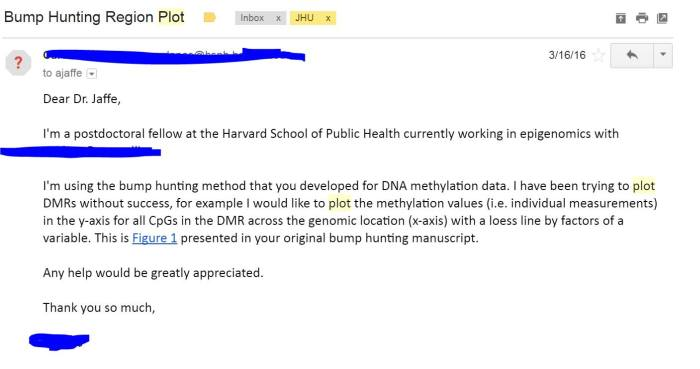
\includegraphics{media/code_request.jpg}
\caption{The paper came out January 2012 with code made in 2011}
\end{figure}

\end{frame}

\begin{frame}{Commenting in Scripts}
\protect\hypertarget{commenting-in-scripts-2}{}

\begin{figure}
\centering
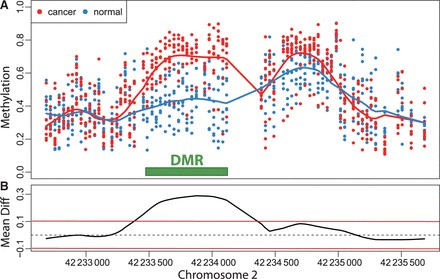
\includegraphics{media/dyr238f1.gif}
\caption{This was the figure\ldots{}}
\end{figure}

\end{frame}

\begin{frame}{Commenting in Scripts}
\protect\hypertarget{commenting-in-scripts-3}{}

\begin{figure}
\centering
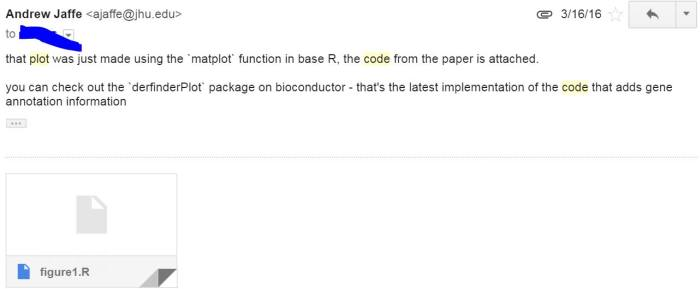
\includegraphics{media/code_fu.jpg}
\caption{After some digging, I found the code}
\end{figure}

\end{frame}

\begin{frame}[fragile]{Commenting in Scripts}
\protect\hypertarget{commenting-in-scripts-4}{}

Add a comment header to your script from today:\texttt{\#} is the
comment symbol

\begin{Shaded}
\begin{Highlighting}[]
\CommentTok{#################}
\CommentTok{# Title: Demo R Script}
\CommentTok{# Author: Andrew Jaffe}
\CommentTok{# Date: 7/15/2019}
\CommentTok{# Purpose: Demonstrate comments in R}
\CommentTok{###################}
 
\CommentTok{# nothing to its right is evaluated}

\CommentTok{# this # is still a comment}
\CommentTok{### you can use many #'s as you want}

\CommentTok{# sometimes you have a really long comment,}
\CommentTok{#    like explaining what you are doing }
\CommentTok{#    for a step in analysis. }
\CommentTok{# Take it to another line}
\end{Highlighting}
\end{Shaded}

\end{frame}

\begin{frame}[fragile]{Data Input}
\protect\hypertarget{data-input-4}{}

Initially-harder-but-gets-way-easier way: Utilizing functions in the
\texttt{readr} package called \texttt{read\_delim()} and
\texttt{read\_csv()} {[}or like \texttt{read.table()} and
\texttt{read.csv()} using base R functions.

\end{frame}

\begin{frame}[fragile]{Data Input}
\protect\hypertarget{data-input-5}{}

So what is going on ``behind the scenes''?

\texttt{read\_delim()}: Read a delimited file into a data frame.

\begin{verbatim}
read_delim(file, delim, quote = "\"", escape_backslash = FALSE,
  escape_double = TRUE, col_names = TRUE, col_types = NULL,
  locale = default_locale(), na = c("", "NA"), quoted_na = TRUE,
  comment = "", trim_ws = FALSE, skip = 0, n_max = Inf,
  guess_max = min(1000, n_max), progress = interactive())
           
# for example: `read_delim("file.txt",delim="\t")`
\end{verbatim}

\end{frame}

\begin{frame}{Data Input}
\protect\hypertarget{data-input-6}{}

\begin{itemize}
\tightlist
\item
  The filename is the path to your file, in quotes
\item
  The function will look in your ``working directory'' if no absolute
  file path is given
\item
  Note that the filename can also be a path to a file on a website
  (e.g.~`www.someurl.com/table1.txt')
\end{itemize}

\end{frame}

\begin{frame}[fragile]{Data Input}
\protect\hypertarget{data-input-7}{}

There is another convenient function for reading in CSV files, where the
delimiter is assumed to be a comma:

\begin{Shaded}
\begin{Highlighting}[]
\NormalTok{read_csv}
\end{Highlighting}
\end{Shaded}

\begin{verbatim}
function (file, col_names = TRUE, col_types = NULL, locale = default_locale(), 
    na = c("", "NA"), quoted_na = TRUE, quote = "\"", comment = "", 
    trim_ws = TRUE, skip = 0, n_max = Inf, guess_max = min(1000, 
        n_max), progress = show_progress(), skip_empty_rows = TRUE) 
{
    tokenizer <- tokenizer_csv(na = na, quoted_na = quoted_na, 
        quote = quote, comment = comment, trim_ws = trim_ws, 
        skip_empty_rows = skip_empty_rows)
    read_delimited(file, tokenizer, col_names = col_names, col_types = col_types, 
        locale = locale, skip = skip, skip_empty_rows = skip_empty_rows, 
        comment = comment, n_max = n_max, guess_max = guess_max, 
        progress = progress)
}
<bytecode: 0x00000000179d8dd8>
<environment: namespace:readr>
\end{verbatim}

\end{frame}

\begin{frame}[fragile]{Data Input}
\protect\hypertarget{data-input-8}{}

\begin{itemize}
\tightlist
\item
  Here would be reading in the data from the command line, specifying
  the file path:
\end{itemize}

\begin{Shaded}
\begin{Highlighting}[]
\NormalTok{ufo =}\StringTok{ }\KeywordTok{read_csv}\NormalTok{(}\StringTok{"../data/ufo/ufo_data_complete.csv"}\NormalTok{)}
\end{Highlighting}
\end{Shaded}

\begin{verbatim}
Parsed with column specification:
cols(
  datetime = col_character(),
  city = col_character(),
  state = col_character(),
  country = col_character(),
  shape = col_character(),
  `duration (seconds)` = col_double(),
  `duration (hours/min)` = col_character(),
  comments = col_character(),
  `date posted` = col_character(),
  latitude = col_character(),
  longitude = col_double()
)
\end{verbatim}

\begin{verbatim}
Warning: 199 parsing failures.
 row col   expected     actual                                file
 877  -- 11 columns 12 columns '../data/ufo/ufo_data_complete.csv'
1712  -- 11 columns 12 columns '../data/ufo/ufo_data_complete.csv'
1814  -- 11 columns 12 columns '../data/ufo/ufo_data_complete.csv'
2857  -- 11 columns 12 columns '../data/ufo/ufo_data_complete.csv'
3733  -- 11 columns 12 columns '../data/ufo/ufo_data_complete.csv'
.... ... .......... .......... ...................................
See problems(...) for more details.
\end{verbatim}

The data is now successfully read into your R workspace, just like from
using the dropdown menu.

\end{frame}

\begin{frame}[fragile]{Data Input}
\protect\hypertarget{data-input-9}{}

The \texttt{read\_delim()} and related functions returns a ``tibble'' is
a \texttt{data.frame} with special printing, which is the primary data
format for most data cleaning and analyses.

\end{frame}

\begin{frame}[fragile]{Data Input with \texttt{tbl\_df}s}
\protect\hypertarget{data-input-with-tbl_dfs}{}

\begin{itemize}
\tightlist
\item
  When using the dropdown menu in RStudio, it uses \texttt{read\_csv},
  which is an improved version of reading in CSVs. It is popular but
  \texttt{read.csv} is still largely used. It returns a \texttt{tbl}
  (tibble), that is a \texttt{data.frame} with improved printing and
  subsetting properties:
\end{itemize}

\begin{Shaded}
\begin{Highlighting}[]
\KeywordTok{head}\NormalTok{(ufo)}
\end{Highlighting}
\end{Shaded}

\begin{verbatim}
# A tibble: 6 x 11
  datetime city  state country shape `duration (seco~ `duration (hour~
  <chr>    <chr> <chr> <chr>   <chr>            <dbl> <chr>           
1 10/10/1~ san ~ tx    us      cyli~             2700 45 minutes      
2 10/10/1~ lack~ tx    <NA>    light             7200 1-2 hrs         
3 10/10/1~ ches~ <NA>  gb      circ~               20 20 seconds      
4 10/10/1~ edna  tx    us      circ~               20 1/2 hour        
5 10/10/1~ kane~ hi    us      light              900 15 minutes      
6 10/10/1~ bris~ tn    us      sphe~              300 5 minutes       
# ... with 4 more variables: comments <chr>, `date posted` <chr>,
#   latitude <chr>, longitude <dbl>
\end{verbatim}

\begin{Shaded}
\begin{Highlighting}[]
\KeywordTok{class}\NormalTok{(ufo)}
\end{Highlighting}
\end{Shaded}

\begin{verbatim}
[1] "spec_tbl_df" "tbl_df"      "tbl"         "data.frame" 
\end{verbatim}

\end{frame}

\begin{frame}[fragile]{Data Input}
\protect\hypertarget{data-input-10}{}

\begin{Shaded}
\begin{Highlighting}[]
\NormalTok{ufo}
\end{Highlighting}
\end{Shaded}

\begin{verbatim}
# A tibble: 88,875 x 11
   datetime city  state country shape `duration (seco~ `duration (hour~
   <chr>    <chr> <chr> <chr>   <chr>            <dbl> <chr>           
 1 10/10/1~ san ~ tx    us      cyli~             2700 45 minutes      
 2 10/10/1~ lack~ tx    <NA>    light             7200 1-2 hrs         
 3 10/10/1~ ches~ <NA>  gb      circ~               20 20 seconds      
 4 10/10/1~ edna  tx    us      circ~               20 1/2 hour        
 5 10/10/1~ kane~ hi    us      light              900 15 minutes      
 6 10/10/1~ bris~ tn    us      sphe~              300 5 minutes       
 7 10/10/1~ pena~ <NA>  gb      circ~              180 about 3 mins    
 8 10/10/1~ norw~ ct    us      disk              1200 20 minutes      
 9 10/10/1~ pell~ al    us      disk               180 3  minutes      
10 10/10/1~ live~ fl    us      disk               120 several minutes 
# ... with 88,865 more rows, and 4 more variables: comments <chr>, `date
#   posted` <chr>, latitude <chr>, longitude <dbl>
\end{verbatim}

\end{frame}

\begin{frame}[fragile]{Data Input}
\protect\hypertarget{data-input-11}{}

There are also data importing functions provided in base R (rather than
the \texttt{readr} package), like \texttt{read.delim} and
\texttt{read.csv}.

These functions have slightly different syntax for reading in data, like
\texttt{header} and \texttt{as.is}.

However, while many online resources use the base R tools, the latest
version of RStudio switched to use these new \texttt{readr} data import
tools, so we will use them in the class for slides. They are also up to
two times faster for reading in large datasets, and have a progress bar
which is nice.

But you can use whatever function you feel more comfortable with.

\end{frame}

\begin{frame}[fragile]{Data Input}
\protect\hypertarget{data-input-12}{}

\begin{itemize}
\tightlist
\item
  Sometimes you get weird messages when reading in data:
\item
  The \texttt{spec()} and \texttt{problems()} functions show you the
  specification of how the data was read in.
\end{itemize}

\begin{Shaded}
\begin{Highlighting}[]
\KeywordTok{dim}\NormalTok{(}\KeywordTok{problems}\NormalTok{(ufo))}
\end{Highlighting}
\end{Shaded}

\begin{verbatim}
[1] 199   5
\end{verbatim}

\begin{Shaded}
\begin{Highlighting}[]
\KeywordTok{spec}\NormalTok{(ufo)}
\end{Highlighting}
\end{Shaded}

\begin{verbatim}
cols(
  datetime = col_character(),
  city = col_character(),
  state = col_character(),
  country = col_character(),
  shape = col_character(),
  `duration (seconds)` = col_double(),
  `duration (hours/min)` = col_character(),
  comments = col_character(),
  `date posted` = col_character(),
  latitude = col_character(),
  longitude = col_double()
)
\end{verbatim}

\end{frame}

\begin{frame}[fragile]{Data Input: Checking for problems}
\protect\hypertarget{data-input-checking-for-problems}{}

\begin{itemize}
\tightlist
\item
  The \texttt{stop\_for\_problems()} function will stop if your data had
  an error when reading in. If this occurs, you can either use
  \texttt{col\_types} (from \texttt{spec()}) for the problematic
  columns, or set \texttt{guess\_max\ =\ Inf} (takes much longer):
\end{itemize}

\begin{Shaded}
\begin{Highlighting}[]
\KeywordTok{stop_for_problems}\NormalTok{(ufo)}
\end{Highlighting}
\end{Shaded}

\end{frame}

\begin{frame}[fragile]{Data Input}
\protect\hypertarget{data-input-13}{}

The \texttt{read\_delim()} and related functions returns a ``tibble'' is
a \texttt{data.frame} with special printing, which is the primary data
format for most data cleaning and analyses.

\end{frame}

\begin{frame}[fragile]{Base R: Data Input}
\protect\hypertarget{base-r-data-input}{}

There are also data importing functions provided in base R (rather than
the \texttt{readr} package), like \texttt{read.delim} and
\texttt{read.csv}.

These functions have slightly different syntax for reading in data, like
\texttt{header} and \texttt{as.is}.

However, while many online resources use the base R tools, the latest
version of RStudio switched to use these new \texttt{readr} data import
tools, so we will use them in the class for slides. They are also up to
two times faster for reading in large datasets, and have a progress bar
which is nice.

But you can use whatever function you feel more comfortable with.

\end{frame}

\begin{frame}[fragile]{Base R: Data Input}
\protect\hypertarget{base-r-data-input-1}{}

Here is how to read in the same dataset using base R functionality,
which returns a \texttt{data.frame} directly

\begin{Shaded}
\begin{Highlighting}[]
\NormalTok{ufo2 =}\StringTok{ }\KeywordTok{read.csv}\NormalTok{(}\StringTok{"../data/ufo/ufo_data_complete.csv"}\NormalTok{, }\DataTypeTok{as.is =} \OtherTok{TRUE}\NormalTok{)}
\KeywordTok{head}\NormalTok{(ufo2)}
\end{Highlighting}
\end{Shaded}

\begin{verbatim}
          datetime                 city state country    shape
1 10/10/1949 20:30           san marcos    tx      us cylinder
2 10/10/1949 21:00         lackland afb    tx            light
3 10/10/1955 17:00 chester (uk/england)            gb   circle
4 10/10/1956 21:00                 edna    tx      us   circle
5 10/10/1960 20:00              kaneohe    hi      us    light
6 10/10/1961 19:00              bristol    tn      us   sphere
  duration..seconds. duration..hours.min.
1               2700           45 minutes
2               7200              1-2 hrs
3                 20           20 seconds
4                 20             1/2 hour
5                900           15 minutes
6                300            5 minutes
                                                                                                                                                    comments
1                    This event took place in early fall around 1949-50. It occurred after a Boy Scout meeting in the Baptist Church. The Baptist Church sit
2                                                            1949 Lackland AFB&#44 TX.  Lights racing across the sky &amp; making 90 degree turns on a dime.
3                                                                                                        Green/Orange circular disc over Chester&#44 England
4                 My older brother and twin sister were leaving the only Edna theater at about 9 PM&#44...we had our bikes and I took a different route home
5 AS a Marine 1st Lt. flying an FJ4B fighter/attack aircraft on a solo night exercise&#44 I was at 50&#44000&#39 in a &quot;clean&quot; aircraft (no ordinan
6                 My father is now 89 my brother 52 the girl with us now 51 myself 49 and the other fellow which worked with my father if he&#39s still livi
  date.posted   latitude   longitude
1   4/27/2004 29.8830556  -97.941111
2  12/16/2005   29.38421  -98.581082
3   1/21/2008       53.2   -2.916667
4   1/17/2004 28.9783333  -96.645833
5   1/22/2004 21.4180556 -157.803611
6   4/27/2007 36.5950000  -82.188889
\end{verbatim}

We will use the \texttt{readr} functionality for certain reasons.

\end{frame}

\begin{frame}[fragile]{More ways to save: write\_rds}
\protect\hypertarget{more-ways-to-save-write_rds}{}

If you want to save \textbf{one} object, you can use
\texttt{readr::write\_rds} to save to an \texttt{rds} file:

\begin{Shaded}
\begin{Highlighting}[]
\KeywordTok{write_rds}\NormalTok{(ufo, }\DataTypeTok{path =} \StringTok{"ufo_dataset.rds"}\NormalTok{)}
\end{Highlighting}
\end{Shaded}

\end{frame}

\begin{frame}[fragile]{More ways to save: read\_rds}
\protect\hypertarget{more-ways-to-save-read_rds}{}

To read this back in to R, you need to use \texttt{read\_rds}, but
\textbf{need to assign it}:

\begin{Shaded}
\begin{Highlighting}[]
\NormalTok{ufo3 =}\StringTok{ }\KeywordTok{read_rds}\NormalTok{(}\DataTypeTok{path =} \StringTok{"ufo_dataset.rds"}\NormalTok{)}
\KeywordTok{identical}\NormalTok{(ufo, ufo3) }\CommentTok{# test if they are the same }
\end{Highlighting}
\end{Shaded}

\begin{verbatim}
[1] TRUE
\end{verbatim}

\end{frame}

\begin{frame}[fragile]{More ways to save: save}
\protect\hypertarget{more-ways-to-save-save}{}

The \texttt{save} command can save a set of \texttt{R} objects into an
``R data file'', with the extension \texttt{.rda} or \texttt{.RData}.

\begin{Shaded}
\begin{Highlighting}[]
\NormalTok{x =}\StringTok{ }\DecValTok{5}
\KeywordTok{save}\NormalTok{(ufo, x, }\DataTypeTok{file =} \StringTok{"ufo_data.rda"}\NormalTok{)}
\end{Highlighting}
\end{Shaded}

\end{frame}

\begin{frame}[fragile]{More ways to save: load}
\protect\hypertarget{more-ways-to-save-load}{}

The opposite of \texttt{save} is \texttt{load}. The \texttt{ls()}
command lists the items in the workspace/environment and \texttt{rm}
removes them:

\end{frame}

\begin{frame}[fragile]{Data Summaries}
\protect\hypertarget{data-summaries}{}

\begin{itemize}
\tightlist
\item
  \texttt{nrow()} displays the number of rows of a data frame
\item
  \texttt{ncol()} displays the number of columns
\item
  \texttt{dim()} displays a vector of length 2: \# rows, \# columns
\end{itemize}

\begin{Shaded}
\begin{Highlighting}[]
\KeywordTok{dim}\NormalTok{(ufo)}
\end{Highlighting}
\end{Shaded}

\begin{verbatim}
[1] 88875    11
\end{verbatim}

\begin{Shaded}
\begin{Highlighting}[]
\KeywordTok{nrow}\NormalTok{(ufo)}
\end{Highlighting}
\end{Shaded}

\begin{verbatim}
[1] 88875
\end{verbatim}

\begin{Shaded}
\begin{Highlighting}[]
\KeywordTok{ncol}\NormalTok{(ufo)}
\end{Highlighting}
\end{Shaded}

\begin{verbatim}
[1] 11
\end{verbatim}

\end{frame}

\begin{frame}[fragile]{Data Summaries}
\protect\hypertarget{data-summaries-1}{}

\begin{itemize}
\tightlist
\item
  \texttt{colnames()} displays the column names (if any) and
  \texttt{rownames()} displays the row names (if any)
\item
  Note that tibbles do not have rownames
\end{itemize}

\begin{Shaded}
\begin{Highlighting}[]
\KeywordTok{colnames}\NormalTok{(ufo)}
\end{Highlighting}
\end{Shaded}

\begin{verbatim}
 [1] "datetime"             "city"                 "state"               
 [4] "country"              "shape"                "duration (seconds)"  
 [7] "duration (hours/min)" "comments"             "date posted"         
[10] "latitude"             "longitude"           
\end{verbatim}

\end{frame}

\hypertarget{data-classes}{%
\section{Data Classes}\label{data-classes}}

\begin{frame}[fragile]{R variables}
\protect\hypertarget{r-variables}{}

\begin{itemize}
\tightlist
\item
  The most comfortable and familiar class/data type for many of you will
  be \texttt{data.frame}
\item
  You can think of these as essentially Excel spreadsheets with rows
  (usually subjects or observations) and columns (usually variables)
\end{itemize}

\end{frame}

\begin{frame}{Data Classes:}
\protect\hypertarget{data-classes-1}{}

\begin{itemize}
\tightlist
\item
  One dimensional classes (`vectors'):

  \begin{itemize}
  \tightlist
  \item
    Character: strings or individual characters, quoted
  \item
    Numeric: any real number(s)
  \item
    Integer: any integer(s)/whole numbers
  \item
    Factor: categorical/qualitative variables
  \item
    Logical: variables composed of TRUE or FALSE
  \item
    Date/POSIXct: represents calendar dates and times
  \end{itemize}
\end{itemize}

\end{frame}

\hypertarget{r-variables-1}{%
\section{R variables}\label{r-variables-1}}

\begin{frame}[fragile]{Numeric}
\protect\hypertarget{numeric}{}

You can perform functions to entire vectors of numbers very easily.

\begin{Shaded}
\begin{Highlighting}[]
\NormalTok{x =}\StringTok{ }\KeywordTok{c}\NormalTok{(}\DecValTok{3}\NormalTok{,}\DecValTok{68}\NormalTok{,}\DecValTok{4}\NormalTok{,}\DecValTok{2}\NormalTok{)}
\NormalTok{x }\OperatorTok{+}\StringTok{ }\DecValTok{2}
\end{Highlighting}
\end{Shaded}

\begin{verbatim}
[1]  5 70  6  4
\end{verbatim}

\begin{Shaded}
\begin{Highlighting}[]
\NormalTok{x }\OperatorTok{*}\StringTok{ }\DecValTok{3}
\end{Highlighting}
\end{Shaded}

\begin{verbatim}
[1]   9 204  12   6
\end{verbatim}

\begin{Shaded}
\begin{Highlighting}[]
\NormalTok{x }\OperatorTok{+}\StringTok{ }\KeywordTok{c}\NormalTok{(}\DecValTok{1}\NormalTok{, }\DecValTok{2}\NormalTok{, }\DecValTok{3}\NormalTok{, }\DecValTok{4}\NormalTok{)}
\end{Highlighting}
\end{Shaded}

\begin{verbatim}
[1]  4 70  7  6
\end{verbatim}

\end{frame}

\begin{frame}[fragile]{R variables}
\protect\hypertarget{r-variables-2}{}

But things like algebra can only be performed on numbers.

\begin{verbatim}
> c("Andrew", "Jaffe") + 4
[1] Error in name2 * 4 : non-numeric argument
 to binary operator
\end{verbatim}

\end{frame}

\begin{frame}[fragile]{R variables}
\protect\hypertarget{r-variables-3}{}

And save these modified vectors as a new vector.

\begin{Shaded}
\begin{Highlighting}[]
\NormalTok{y =}\StringTok{ "Hello World"}
\NormalTok{y}
\end{Highlighting}
\end{Shaded}

\begin{verbatim}
[1] "Hello World"
\end{verbatim}

\begin{Shaded}
\begin{Highlighting}[]
\NormalTok{y =}\StringTok{ }\NormalTok{x }\OperatorTok{+}\StringTok{ }\KeywordTok{c}\NormalTok{(}\DecValTok{1}\NormalTok{, }\DecValTok{2}\NormalTok{, }\DecValTok{3}\NormalTok{, }\DecValTok{4}\NormalTok{)}
\NormalTok{y }
\end{Highlighting}
\end{Shaded}

\begin{verbatim}
[1]  4 70  7  6
\end{verbatim}

Note that the R object \texttt{y} is no longer ``Hello World!'' - It has
effectively been overwritten by assigning new data to the variable

\end{frame}

\begin{frame}[fragile]{R variables}
\protect\hypertarget{r-variables-4}{}

\begin{itemize}
\tightlist
\item
  You can get more attributes than just class. The function \texttt{str}
  gives you the structure of the object.
\end{itemize}

\begin{Shaded}
\begin{Highlighting}[]
\KeywordTok{class}\NormalTok{(x)}
\end{Highlighting}
\end{Shaded}

\begin{verbatim}
[1] "numeric"
\end{verbatim}

\begin{Shaded}
\begin{Highlighting}[]
\KeywordTok{str}\NormalTok{(x)}
\end{Highlighting}
\end{Shaded}

\begin{verbatim}
 num [1:4] 3 68 4 2
\end{verbatim}

This tells you that \texttt{x} is a numeric vector and tells you the
length.

\end{frame}

\begin{frame}[fragile]{Logical}
\protect\hypertarget{logical}{}

\texttt{logical} is a class that only has two possible elements:
\texttt{TRUE} and \texttt{FALSE}

\begin{Shaded}
\begin{Highlighting}[]
\NormalTok{x =}\StringTok{ }\KeywordTok{c}\NormalTok{(}\OtherTok{TRUE}\NormalTok{, }\OtherTok{FALSE}\NormalTok{, }\OtherTok{TRUE}\NormalTok{, }\OtherTok{TRUE}\NormalTok{, }\OtherTok{FALSE}\NormalTok{)}
\KeywordTok{class}\NormalTok{(x)}
\end{Highlighting}
\end{Shaded}

\begin{verbatim}
[1] "logical"
\end{verbatim}

\begin{Shaded}
\begin{Highlighting}[]
\KeywordTok{is.numeric}\NormalTok{(}\KeywordTok{c}\NormalTok{(}\StringTok{"Andrew"}\NormalTok{, }\StringTok{"Jaffe"}\NormalTok{))}
\end{Highlighting}
\end{Shaded}

\begin{verbatim}
[1] FALSE
\end{verbatim}

\begin{Shaded}
\begin{Highlighting}[]
\KeywordTok{is.character}\NormalTok{(}\KeywordTok{c}\NormalTok{(}\StringTok{"Andrew"}\NormalTok{, }\StringTok{"Jaffe"}\NormalTok{))}
\end{Highlighting}
\end{Shaded}

\begin{verbatim}
[1] TRUE
\end{verbatim}

\end{frame}

\begin{frame}[fragile]{Logical}
\protect\hypertarget{logical-1}{}

Note that \texttt{logical} elements are NOT in quotes.

\begin{Shaded}
\begin{Highlighting}[]
\NormalTok{z =}\StringTok{ }\KeywordTok{c}\NormalTok{(}\StringTok{"TRUE"}\NormalTok{, }\StringTok{"FALSE"}\NormalTok{, }\StringTok{"TRUE"}\NormalTok{, }\StringTok{"FALSE"}\NormalTok{)}
\KeywordTok{class}\NormalTok{(z)}
\end{Highlighting}
\end{Shaded}

\begin{verbatim}
[1] "character"
\end{verbatim}

\begin{Shaded}
\begin{Highlighting}[]
\KeywordTok{as.logical}\NormalTok{(z)}
\end{Highlighting}
\end{Shaded}

\begin{verbatim}
[1]  TRUE FALSE  TRUE FALSE
\end{verbatim}

Bonus: \texttt{sum()} and \texttt{mean()} work on \texttt{logical}
vectors - they return the total and proportion of \texttt{TRUE}
elements, respectively.

\begin{Shaded}
\begin{Highlighting}[]
\KeywordTok{sum}\NormalTok{(}\KeywordTok{as.logical}\NormalTok{(z))}
\end{Highlighting}
\end{Shaded}

\begin{verbatim}
[1] 2
\end{verbatim}

\end{frame}

\begin{frame}[fragile]{General Class Information}
\protect\hypertarget{general-class-information}{}

There are two useful functions associated with practically all R
classes, which relate to logically checking the underlying class
(\texttt{is.CLASS\_()}) and coercing between classes
(\texttt{as.CLASS\_()}).

\begin{Shaded}
\begin{Highlighting}[]
\KeywordTok{is.numeric}\NormalTok{(}\KeywordTok{c}\NormalTok{(}\StringTok{"Andrew"}\NormalTok{, }\StringTok{"Jaffe"}\NormalTok{))}
\end{Highlighting}
\end{Shaded}

\begin{verbatim}
[1] FALSE
\end{verbatim}

\begin{Shaded}
\begin{Highlighting}[]
\KeywordTok{is.character}\NormalTok{(}\KeywordTok{c}\NormalTok{(}\StringTok{"Andrew"}\NormalTok{, }\StringTok{"Jaffe"}\NormalTok{))}
\end{Highlighting}
\end{Shaded}

\begin{verbatim}
[1] TRUE
\end{verbatim}

\end{frame}

\begin{frame}[fragile]{General Class Information}
\protect\hypertarget{general-class-information-1}{}

There are two useful functions associated with practically all R
classes, which relate to logically checking the underlying class
(\texttt{is.CLASS\_()}) and coercing between classes
(\texttt{as.CLASS\_()}).

\begin{Shaded}
\begin{Highlighting}[]
\KeywordTok{as.character}\NormalTok{(}\KeywordTok{c}\NormalTok{(}\DecValTok{1}\NormalTok{, }\DecValTok{4}\NormalTok{, }\DecValTok{7}\NormalTok{))}
\end{Highlighting}
\end{Shaded}

\begin{verbatim}
[1] "1" "4" "7"
\end{verbatim}

\begin{Shaded}
\begin{Highlighting}[]
\KeywordTok{as.numeric}\NormalTok{(}\KeywordTok{c}\NormalTok{(}\StringTok{"Andrew"}\NormalTok{, }\StringTok{"Jaffe"}\NormalTok{))}
\end{Highlighting}
\end{Shaded}

\begin{verbatim}
Warning: NAs introduced by coercion
\end{verbatim}

\begin{verbatim}
[1] NA NA
\end{verbatim}

\end{frame}

\begin{frame}[fragile]{Factors}
\protect\hypertarget{factors}{}

A \texttt{factor} is a special \texttt{character} vector where the
elements have pre-defined groups or `levels'. You can think of these as
qualitative or categorical variables:

\begin{Shaded}
\begin{Highlighting}[]
\NormalTok{x =}\StringTok{ }\KeywordTok{factor}\NormalTok{(}\KeywordTok{c}\NormalTok{(}\StringTok{"boy"}\NormalTok{, }\StringTok{"girl"}\NormalTok{, }\StringTok{"girl"}\NormalTok{, }\StringTok{"boy"}\NormalTok{, }\StringTok{"girl"}\NormalTok{))}
\NormalTok{x }
\end{Highlighting}
\end{Shaded}

\begin{verbatim}
[1] boy  girl girl boy  girl
Levels: boy girl
\end{verbatim}

\begin{Shaded}
\begin{Highlighting}[]
\KeywordTok{class}\NormalTok{(x)}
\end{Highlighting}
\end{Shaded}

\begin{verbatim}
[1] "factor"
\end{verbatim}

Note that levels are, by default, in alphanumerical order.

\end{frame}

\begin{frame}[fragile]{Factors}
\protect\hypertarget{factors-1}{}

Factors are used to represent categorical data, and can also be used for
ordinal data (ie categories have an intrinsic ordering)

Note that R reads in character strings as factors by default in
functions like \texttt{read.table()}

`The function factor is used to encode a vector as a factor (the terms
'category' and `enumerated type' are also used for factors). If argument
ordered is TRUE, the factor levels are assumed to be ordered.'

\begin{verbatim}
factor(x = character(), levels, labels = levels,
       exclude = NA, ordered = is.ordered(x))
\end{verbatim}

\end{frame}

\begin{frame}[fragile]{Factors}
\protect\hypertarget{factors-2}{}

Suppose we have a vector of case-control status

\begin{Shaded}
\begin{Highlighting}[]
\NormalTok{cc =}\StringTok{ }\KeywordTok{factor}\NormalTok{(}\KeywordTok{c}\NormalTok{(}\StringTok{"case"}\NormalTok{,}\StringTok{"case"}\NormalTok{,}\StringTok{"case"}\NormalTok{,}
        \StringTok{"control"}\NormalTok{,}\StringTok{"control"}\NormalTok{,}\StringTok{"control"}\NormalTok{))}
\NormalTok{cc}
\end{Highlighting}
\end{Shaded}

\begin{verbatim}
[1] case    case    case    control control control
Levels: case control
\end{verbatim}

\begin{Shaded}
\begin{Highlighting}[]
\KeywordTok{levels}\NormalTok{(cc) =}\StringTok{ }\KeywordTok{c}\NormalTok{(}\StringTok{"control"}\NormalTok{,}\StringTok{"case"}\NormalTok{)}
\NormalTok{cc}
\end{Highlighting}
\end{Shaded}

\begin{verbatim}
[1] control control control case    case    case   
Levels: control case
\end{verbatim}

\end{frame}

\begin{frame}[fragile]{Factors}
\protect\hypertarget{factors-3}{}

Note that the levels are alphabetically ordered by default. We can also
specify the levels within the factor call

\begin{Shaded}
\begin{Highlighting}[]
\NormalTok{casecontrol =}\StringTok{ }\KeywordTok{c}\NormalTok{(}\StringTok{"case"}\NormalTok{,}\StringTok{"case"}\NormalTok{,}\StringTok{"case"}\NormalTok{,}\StringTok{"control"}\NormalTok{,}
          \StringTok{"control"}\NormalTok{,}\StringTok{"control"}\NormalTok{)}
\KeywordTok{factor}\NormalTok{(casecontrol, }\DataTypeTok{levels =} \KeywordTok{c}\NormalTok{(}\StringTok{"control"}\NormalTok{,}\StringTok{"case"}\NormalTok{) )}
\end{Highlighting}
\end{Shaded}

\begin{verbatim}
[1] case    case    case    control control control
Levels: control case
\end{verbatim}

\begin{Shaded}
\begin{Highlighting}[]
\KeywordTok{factor}\NormalTok{(casecontrol, }\DataTypeTok{levels =} \KeywordTok{c}\NormalTok{(}\StringTok{"control"}\NormalTok{,}\StringTok{"case"}\NormalTok{), }
       \DataTypeTok{ordered=}\OtherTok{TRUE}\NormalTok{)}
\end{Highlighting}
\end{Shaded}

\begin{verbatim}
[1] case    case    case    control control control
Levels: control < case
\end{verbatim}

\end{frame}

\begin{frame}[fragile]{Factors}
\protect\hypertarget{factors-4}{}

Factors can be converted to \texttt{numeric} or \texttt{character} very
easily

\begin{Shaded}
\begin{Highlighting}[]
\NormalTok{x =}\StringTok{ }\KeywordTok{factor}\NormalTok{(casecontrol,}
        \DataTypeTok{levels =} \KeywordTok{c}\NormalTok{(}\StringTok{"control"}\NormalTok{,}\StringTok{"case"}\NormalTok{) )}
\KeywordTok{as.character}\NormalTok{(x)}
\end{Highlighting}
\end{Shaded}

\begin{verbatim}
[1] "case"    "case"    "case"    "control" "control" "control"
\end{verbatim}

\begin{Shaded}
\begin{Highlighting}[]
\KeywordTok{as.numeric}\NormalTok{(x)}
\end{Highlighting}
\end{Shaded}

\begin{verbatim}
[1] 2 2 2 1 1 1
\end{verbatim}

\end{frame}

\begin{frame}[fragile]{Factors}
\protect\hypertarget{factors-5}{}

However, you need to be careful modifying the labels of existing
factors, as its quite easy to alter the meaning of the underlying data.

\begin{Shaded}
\begin{Highlighting}[]
\NormalTok{xCopy =}\StringTok{ }\NormalTok{x}
\KeywordTok{levels}\NormalTok{(xCopy) =}\StringTok{ }\KeywordTok{c}\NormalTok{(}\StringTok{"case"}\NormalTok{, }\StringTok{"control"}\NormalTok{) }\CommentTok{# wrong way}
\NormalTok{xCopy        }
\end{Highlighting}
\end{Shaded}

\begin{verbatim}
[1] control control control case    case    case   
Levels: case control
\end{verbatim}

\begin{Shaded}
\begin{Highlighting}[]
\KeywordTok{as.character}\NormalTok{(xCopy) }\CommentTok{# labels switched}
\end{Highlighting}
\end{Shaded}

\begin{verbatim}
[1] "control" "control" "control" "case"    "case"    "case"   
\end{verbatim}

\begin{Shaded}
\begin{Highlighting}[]
\KeywordTok{as.numeric}\NormalTok{(xCopy)}
\end{Highlighting}
\end{Shaded}

\begin{verbatim}
[1] 2 2 2 1 1 1
\end{verbatim}

\end{frame}

\begin{frame}[fragile]{Date}
\protect\hypertarget{date}{}

You can convert date-like strings in the \texttt{Date} class
(\url{http://www.statmethods.net/input/dates.html} for more info)

\begin{Shaded}
\begin{Highlighting}[]
\NormalTok{theDate =}\StringTok{ }\KeywordTok{c}\NormalTok{(}\StringTok{"01/21/1990"}\NormalTok{, }\StringTok{"02/01/1989"}\NormalTok{, }\StringTok{"03/23/1988"}\NormalTok{)}
\KeywordTok{sort}\NormalTok{(theDate)}
\end{Highlighting}
\end{Shaded}

\begin{verbatim}
[1] "01/21/1990" "02/01/1989" "03/23/1988"
\end{verbatim}

\begin{Shaded}
\begin{Highlighting}[]
\NormalTok{newDate <-}\StringTok{ }\KeywordTok{as.Date}\NormalTok{(theDate, }\StringTok{"%m/%d/%Y"}\NormalTok{)}
\KeywordTok{sort}\NormalTok{(newDate)}
\end{Highlighting}
\end{Shaded}

\begin{verbatim}
[1] "1988-03-23" "1989-02-01" "1990-01-21"
\end{verbatim}

\end{frame}

\begin{frame}[fragile]{Date}
\protect\hypertarget{date-1}{}

However, the \texttt{lubridate} package is much easier for generating
explicit dates:

\begin{Shaded}
\begin{Highlighting}[]
\KeywordTok{library}\NormalTok{(lubridate) }\CommentTok{# great for dates!}
\NormalTok{newDate2 =}\StringTok{ }\KeywordTok{mdy}\NormalTok{(theDate)}
\NormalTok{newDate2}
\end{Highlighting}
\end{Shaded}

\begin{verbatim}
[1] "1990-01-21" "1989-02-01" "1988-03-23"
\end{verbatim}

\end{frame}

\begin{frame}[fragile]{POSIXct}
\protect\hypertarget{posixct}{}

The \texttt{POSIXct} class is like a more general date format (with
hours, minutes, seconds).

\begin{Shaded}
\begin{Highlighting}[]
\NormalTok{theTime =}\StringTok{ }\KeywordTok{Sys.time}\NormalTok{()}
\NormalTok{theTime}
\end{Highlighting}
\end{Shaded}

\begin{verbatim}
[1] "2019-07-15 08:28:12 PDT"
\end{verbatim}

\begin{Shaded}
\begin{Highlighting}[]
\KeywordTok{class}\NormalTok{(theTime)}
\end{Highlighting}
\end{Shaded}

\begin{verbatim}
[1] "POSIXct" "POSIXt" 
\end{verbatim}

\begin{Shaded}
\begin{Highlighting}[]
\NormalTok{theTime }\OperatorTok{+}\StringTok{ }\KeywordTok{as.period}\NormalTok{(}\DecValTok{20}\NormalTok{, }\DataTypeTok{unit =} \StringTok{"minutes"}\NormalTok{) }\CommentTok{# the future}
\end{Highlighting}
\end{Shaded}

\begin{verbatim}
[1] "2019-07-15 08:48:12 PDT"
\end{verbatim}

\end{frame}

\begin{frame}[fragile]{Data Classes:}
\protect\hypertarget{data-classes-2}{}

\begin{itemize}
\tightlist
\item
  Two dimensional classes:

  \begin{itemize}
  \tightlist
  \item
    \texttt{data.frame}: traditional `Excel' spreadsheets

    \begin{itemize}
    \tightlist
    \item
      Each column can have a different class, from above
    \end{itemize}
  \item
    Matrix: two-dimensional data, composed of rows and columns. Unlike
    data frames, the entire matrix is composed of one R class, e.g.~all
    numeric or all characters.
  \end{itemize}
\end{itemize}

\end{frame}

\begin{frame}[fragile]{Matrix (and Data frame) Functions}
\protect\hypertarget{matrix-and-data-frame-functions}{}

These are in addition to the previous useful vector functions:

\begin{itemize}
\tightlist
\item
  \texttt{nrow()} displays the number of rows of a matrix or data frame
\item
  \texttt{ncol()} displays the number of columns
\item
  \texttt{dim()} displays a vector of length 2: \# rows, \# columns
\item
  \texttt{colnames()} displays the column names (if any) and
  \texttt{rownames()} displays the row names (if any)
\end{itemize}

\end{frame}

\begin{frame}[fragile]{Data Frames}
\protect\hypertarget{data-frames}{}

The \texttt{data.frame} is the other two dimensional variable class.

Again, data frames are like matrices, but each column is a vector that
can have its own class. So some columns might be \texttt{character} and
others might be \texttt{numeric}, while others maybe a \texttt{factor}.

\end{frame}

\begin{frame}[fragile]{Lists}
\protect\hypertarget{lists}{}

\begin{itemize}
\tightlist
\item
  One other data type that is the most generic are \texttt{lists}.
\item
  Can be created using \texttt{list()}
\item
  Can hold vectors, strings, matrices, models, list of other list, lists
  upon lists!
\end{itemize}

\begin{Shaded}
\begin{Highlighting}[]
\OperatorTok{>}\StringTok{ }\NormalTok{mylist <-}\StringTok{ }\KeywordTok{list}\NormalTok{(}\DataTypeTok{letters=}\KeywordTok{c}\NormalTok{(}\StringTok{"A"}\NormalTok{, }\StringTok{"b"}\NormalTok{, }\StringTok{"c"}\NormalTok{), }
\OperatorTok{+}\StringTok{         }\DataTypeTok{numbers=}\DecValTok{1}\OperatorTok{:}\DecValTok{3}\NormalTok{, }\KeywordTok{matrix}\NormalTok{(}\DecValTok{1}\OperatorTok{:}\DecValTok{25}\NormalTok{, }\DataTypeTok{ncol=}\DecValTok{5}\NormalTok{))}
\OperatorTok{>}\StringTok{ }\NormalTok{mylist}
\end{Highlighting}
\end{Shaded}

\begin{verbatim}
$letters
[1] "A" "b" "c"

$numbers
[1] 1 2 3

[[3]]
     [,1] [,2] [,3] [,4] [,5]
[1,]    1    6   11   16   21
[2,]    2    7   12   17   22
[3,]    3    8   13   18   23
[4,]    4    9   14   19   24
[5,]    5   10   15   20   25
\end{verbatim}

\end{frame}

\begin{frame}[fragile]{More on Data Frames}
\protect\hypertarget{more-on-data-frames}{}

\begin{Shaded}
\begin{Highlighting}[]
\KeywordTok{colnames}\NormalTok{(ufo) }\CommentTok{# column names}
\end{Highlighting}
\end{Shaded}

\begin{verbatim}
 [1] "datetime"             "city"                 "state"               
 [4] "country"              "shape"                "duration (seconds)"  
 [7] "duration (hours/min)" "comments"             "date posted"         
[10] "latitude"             "longitude"           
\end{verbatim}

\begin{Shaded}
\begin{Highlighting}[]
\KeywordTok{head}\NormalTok{(ufo}\OperatorTok{$}\NormalTok{city) }\CommentTok{# first few rows}
\end{Highlighting}
\end{Shaded}

\begin{verbatim}
[1] "san marcos"           "lackland afb"         "chester (uk/england)"
[4] "edna"                 "kaneohe"              "bristol"             
\end{verbatim}

\end{frame}

\begin{frame}[fragile]{Data Output}
\protect\hypertarget{data-output}{}

While its nice to be able to read in a variety of data formats, it's
equally important to be able to output data somewhere.

\texttt{write.table()}: prints its required argument \texttt{x} (after
converting it to a \texttt{data.frame} if it is not one nor a
\texttt{matrix}) to a file or connection.

\begin{verbatim}
write.table(x,file = "", append = FALSE, quote = TRUE, sep = " ",
            eol = "\n", na = "NA", dec = ".", row.names = TRUE,
            col.names = TRUE, qmethod = c("escape", "double"),
            fileEncoding = "")
\end{verbatim}

\end{frame}

\begin{frame}[fragile]{Data Output}
\protect\hypertarget{data-output-1}{}

\texttt{x}: the R \texttt{data.frame} or \texttt{matrix} you want to
write

\texttt{file}: the file name where you want to R object written. It can
be an absolute path, or a filename (which writes the file to your
working directory)

\texttt{sep}: what character separates the columns?

\begin{itemize}
\tightlist
\item
  ``,'' = .csv - Note there is also a \texttt{write.csv()} function
\item
  "\t" = tab delimited
\end{itemize}

\texttt{row.names}: I like setting this to FALSE because I email these
to collaborators who open them in Excel

\end{frame}

\begin{frame}[fragile]{Data Output}
\protect\hypertarget{data-output-2}{}

For example, we can write back out the Monuments dataset with the new
column name:

\begin{Shaded}
\begin{Highlighting}[]
\KeywordTok{write.csv}\NormalTok{(ufo[}\DecValTok{1}\OperatorTok{:}\DecValTok{100}\NormalTok{,], }\DataTypeTok{file=}\StringTok{"ufo_first100.csv"}\NormalTok{, }\DataTypeTok{row.names=}\OtherTok{FALSE}\NormalTok{)}
\end{Highlighting}
\end{Shaded}

Note that \texttt{row.names=TRUE} would make the first column contain
the row names, here just the numbers \texttt{1:nrow(mon)}, which is not
very useful for Excel. Note that row names can be useful/informative in
R if they contain information (but then they would just be a separate
column).

\end{frame}

\begin{frame}[fragile]{Data Input - Excel}
\protect\hypertarget{data-input---excel}{}

Many data analysts collaborate with researchers who use Excel to enter
and curate their data. Often times, this is the input data for an
analysis. You therefore have two options for getting this data into R:

\begin{itemize}
\tightlist
\item
  Saving the Excel sheet as a .csv file, and using \texttt{read.csv()}
\item
  Using an add-on package, like \texttt{readxl}
\end{itemize}

For single worksheet .xlsx files, I often just save the spreadsheet as a
.csv file (because I often have to strip off additional summary data
from the columns)

For an .xlsx file with multiple well-formated worksheets, I use the
\texttt{readxl}package for reading in the data.

\end{frame}

\begin{frame}{Data Input - Other Software}
\protect\hypertarget{data-input---other-software}{}

\begin{itemize}
\tightlist
\item
  \textbf{haven} package
  (\url{https://cran.r-project.org/web/packages/haven/index.html}) reads
  in SAS, SPSS, Stata formats
\item
  \textbf{sas7bdat} reads .sas7bdat files
\item
  \textbf{foreign} package - can read all the formats as \textbf{haven}.
  Around longer (aka more testing), but not as maintained (bad for
  future).
\end{itemize}

\end{frame}

\end{document}
